\chapter{Conditionals and recursion}


\section{Boolean expressions}
\index{boolean}
\index{expression!boolean}

Most of the operations we have seen produce results that are
the same type as their operands.  For example, the {\tt +} operator
takes two {\tt int}s and produces an {\tt int}, or two {\tt double}s
and produces a {\tt double}, etc.

\index{operator!relational}
\index{relational operator}

The exceptions we have seen are the {\bf relational operators}, which
compare {\tt int}s and {\tt float}s and return either {\tt true} or
{\tt false}.  {\tt true} and {\tt false} are special values in Java,
and together they make up a type called {\bf boolean}.  You might
recall that when I defined a type, I said it was a set of values.  In
the case of {\tt int}s, {\tt double}s and {\tt String}s, those sets
are pretty big.  For {\tt boolean}s, there are only two values.

Boolean expressions and variables work just like other types of
expressions and variables:

\begin{code}
    boolean flag;
    flag = true;
    boolean testResult = false;
\end{code}

The first example is a simple variable declaration;
the second example is an assignment, and the third example is an
initialization.

The values {\tt true} and {\tt false}
are keywords in Java, so they may appear in a different color,
depending on your development environment.

\index{initialization}
\index{statement!initialization}

The result of a conditional operator is a boolean,
so you can store the result of a comparison in a variable:

\begin{code}
    boolean evenFlag = (n%2 == 0);     // true if n is even
    boolean positiveFlag = (x > 0);    // true if x is positive
\end{code}

and then use it as part of a conditional statement later:

\begin{code}
    if (evenFlag) {
      System.out.println("n was even when I checked it");
    }
\end{code}

A variable used in this way is called a {\bf flag}
because it flags the presence or absence of some condition.


\section{Logical operators}
\index{logical operator}
\index{operator!logical}

There are three {\bf logical operators} in Java: AND, OR and NOT,
which are denoted by the symbols {\tt \&\&}, {\tt ||} and
{\tt !}.  The semantics of these operators is similar
to their meaning in English.  For example {\tt x > 0 \&\& x < 10}
is true only if {\tt x} is greater than zero AND less than 10.
\index{semantics}

{\tt evenFlag || n\%3 == 0} is true if {\em either} of
the conditions is true, that is, if {\tt evenFlag} is true OR the
number is divisible by 3.

Finally, the NOT operator inverts a boolean expression, so {\tt
  !evenFlag} is true if {\tt evenFlag} is false---if the number is
odd.

\index{nested structure}

Logical operators can simplify nested
conditional statements.  For example, can you re-write
this code using a single conditional?

\begin{code}
    if (x > 0) {
      if (x < 10) {
        System.out.println("x is a positive single digit.");
      }
    }
\end{code}


\section{Conditional execution}
\index{conditional}
\index{statement!conditional}

To write useful programs, we almost always need
to check conditions and change the behavior of the program
accordingly.  {\bf Conditional statements} give us this ability.  The
simplest form is the {\tt if} statement:

\begin{code}
    if (x > 0) {
      System.out.println("x is positive");
    }
\end{code}

The expression in parentheses is called the condition.
If it is true, then the statements in brackets get executed.
If the condition is not true, nothing happens.

\index{operator!comparison}
\index{operator!relational}
\index{comparison!operator}
\index{relational operator}

The condition can contain any of the comparison operators,
sometimes called {\bf relational operators}:

\begin{code}
    x == y               // x equals y
    x != y               // x is not equal to y
    x > y                // x is greater than y
    x < y                // x is less than y
    x >= y               // x is greater than or equal to y
    x <= y               // x is less than or equal to y
\end{code}

Although these operations are probably familiar to you, the
syntax Java uses is a little different from mathematical
symbols like $=$, $\neq$ and $\le$.  A common error is
to use a single {\tt =} instead of a double {\tt ==}.  Remember
that {\tt =} is the assignment operator, and {\tt ==} is
a comparison operator.  Also, there is no such thing as
{\tt =<} or {\tt =>}.

The two sides of a condition operator have to be the same
type.  You can only compare {\tt ints} to {\tt ints} and
{\tt doubles} to {\tt doubles}.

The operators {\tt ==} and {\tt !=} work with Strings, but they
don't do what you expect.  And the other relational operators
don't do anything at all.
We will see how to compare strings Section~\ref{incomparable}.


\section{Alternative execution}
\label{alternative}
\index{conditional!alternative}

A second form of conditional execution is alternative execution,
in which there are two possibilities, and the condition determines
which one gets executed.  The syntax looks like:

\begin{code}
    if (x%2 == 0) {
      System.out.println("x is even");
    } else {
      System.out.println("x is odd");
    }
\end{code}

If the remainder when {\tt x} is divided by 2 is zero, then
we know that {\tt x} is even, and this code prints a message
to that effect.  If the condition is false, the second
print statement is executed.  Since the condition must
be true or false, exactly one of the alternatives will be
executed.

As an aside, if you think you might want to check the parity
(evenness or oddness) of numbers often, you might want to
``wrap'' this code up in a method, as follows:

\begin{code}
  public static void printParity(int x) {
    if (x%2 == 0) {
      System.out.println("x is even");
    } else {
      System.out.println("x is odd");
    }
  }
\end{code}

Now you have a method named {\tt printParity} that will print
an appropriate message for any integer you care to provide.
In {\tt main} you would invoke this method like this:

\begin{code}
    printParity(17);
\end{code}

Always remember that when you {\em invoke} a method, you do
not have to declare the types of the arguments you provide.
Java can figure out what type they are.  You should resist the
temptation to write things like:

\begin{code}
    int number = 17;
    printParity(int number);         // WRONG!!!
\end{code}


\section{Chained conditionals}
\index{conditional!chained}

Sometimes you want to check for a number of related conditions
and choose one of several actions.  One way to do this is by
{\bf chaining} a series of {\tt if}s and {\tt else}s:

\begin{code}
    if (x > 0) {
      System.out.println("x is positive");
    } else if (x < 0) {
      System.out.println("x is negative");
    } else {
      System.out.println("x is zero");
    }
\end{code}

These chains can be as long as you want, although they can
be difficult to read if they get out of hand.  One way to
make them easier to read is to use standard indentation,
as demonstrated in these examples.  If you keep all the
statements and squiggly-brackets lined up, you are less
likely to make syntax errors and more likely to find them
if you do.


\section{Nested conditionals}
\index{conditional!nested}

In addition to chaining, you can also nest one conditional
within another.  We could have written the previous example
as:

\begin{code}
    if (x == 0) {
      System.out.println("x is zero");
    } else {
      if (x > 0) {
        System.out.println("x is positive");
      } else {
        System.out.println("x is negative");
      }
    }
\end{code}

There is now an outer conditional that contains two branches.  The
first branch contains a simple {\tt print} statement, but the second
branch contains another conditional statement, which has two branches
of its own.  Those two branches are both {\tt print}
statements, but they could have been conditional statements as
well.

Indentation helps make the structure
apparent, but nevertheless, nested conditionals get difficult to read
very quickly.  Avoid them when you can.
\index{nested structure}

On the other hand, this kind of {\bf nested structure} is common, and
we will see it again, so you better get used to it.


\section{The return statement}
\index{return}
\index{statement!return}

The {\tt return} statement allows you to terminate the execution
of a method before you reach the end.  One reason to use it
is if you detect an error condition:

\begin{code}
  public static void printLogarithm(double x) {
    if (x <= 0.0) {
      System.out.println("Positive numbers only, please.");
      return;
    }

    double result = Math.log(x);
    System.out.println("The log of x is " + result);
  }
\end{code}

This defines a method named {\tt printLogarithm} that takes a
{\tt  double} named {\tt x} as a parameter.  It checks whether
{\tt  x} is less than or equal to zero, in which case it prints an error
message and then uses {\tt return} to exit the method.  The flow of
execution immediately returns to the caller and the remaining lines of
the method are not executed.

I used a floating-point value on the right side of the condition
because there is a floating-point variable on the left.


\section{Type conversion}
\index{type!conversion}
\index{typecasting}

You might wonder how you can get away with an expression like {\tt
"The log of x is " + result}, since one of the operands is a {\tt String}
and the other is a {\tt double}.  In this case Java is being
smart on our behalf, automatically converting the {\tt double} to a
{\tt String} before it does the string concatenation.

%This kind of feature is an example of a common problem in designing a
%programming language, which is that there is a conflict between {\em
%formalism}, which is the requirement that formal languages should have
%simple rules with few exceptions, and {\em convenience}, which is the
%requirement that programming languages be easy to use in practice.

%More often than not, convenience wins, which is usually good for
%expert programmers (who are spared from rigorous but unwieldy
%formalism), but bad for beginning programmers, who are often baffled
%by the complexity of the rules and the number of exceptions.  In this
%book I have tried to simplify things by emphasizing the rules and
%omitting many of the exceptions.

Whenever you try to ``add'' two
expressions, if one of them is a {\tt String}, Java converts the
other to a {\tt String} and then perform string concatenation.  What do you
think happens if you perform an operation between an integer and a
floating-point value?


\section{Recursion}
\label{recursion}
\index{recursion}

I mentioned in the last chapter that it is legal for one method to
invoke another, and we have seen several examples.  I neglected to
mention that it is also legal for a method to invoke itself.  It may
not be obvious why that is a good thing, but it turns out to be one of
the most magical and interesting things a program can do.

For example, look at the following method:

\begin{code}
  public static void countdown(int n) {
    if (n == 0) {
      System.out.println("Blastoff!");
    } else {
      System.out.println(n);
      countdown(n-1);
    }
  }
\end{code}

The name of the method is {\tt countdown} and it takes a single
integer as a parameter.  If the parameter is zero, it prints
the word ``Blastoff.''  Otherwise, it prints the number and
then invokes a method named {\tt countdown}---itself---passing
{\tt n-1} as an argument.

What happens if we invoke this method, in {\tt main}, like
this:

\begin{code}
    countdown(3);
\end{code}

The execution of {\tt countdown} begins with {\tt n=3}, and
since {\tt n} is not zero, it prints the value 3, and then
invokes itself...

\begin{quote}
The execution of {\tt countdown} begins with {\tt n=2}, and
since {\tt n} is not zero, it prints the value 2, and then
invokes itself...

\begin{quote}
The execution of {\tt countdown} begins with {\tt n=1}, and
since {\tt n} is not zero, it prints the value 1, and then
invokes itself...

\begin{quote}
The execution of {\tt countdown} begins with {\tt n=0}, and
since {\tt n} is zero, it prints the word ``Blastoff!''
and then returns.
\end{quote}

The {\tt countdown} that got {\tt n=1} returns.

\end{quote}

The {\tt countdown} that got {\tt n=2} returns.

\end{quote}

The {\tt countdown} that got {\tt n=3} returns.

\noindent And then you're back in {\tt main}.  So the
total output looks like:

\begin{stdout}
3
2
1
Blastoff!
\end{stdout}

As a second example, let's look again at the methods
{\tt newLine} and {\tt threeLine}.

\begin{code}
  public static void newLine() {
    System.out.println("");
  }

  public static void threeLine() {
    newLine();  newLine();  newLine();
  }
\end{code}

Although these work, they would not be much help if we wanted
to print 2 newlines, or 106.  A better alternative would be

\begin{code}
  public static void nLines(int n) {
    if (n > 0) {
      System.out.println("");
      nLines(n-1);
    }
  }
\end{code}

This program similar to {\tt countdown}; as long as {\tt n} is greater
than zero, it prints a newline and then invokes itself to
print {\tt n-1} additional newlines.  The total number
of newlines that get printed is {\tt 1 +(n-1)}, which usually
comes out to roughly {\tt n}.

\index{recursive}
\index{newline}

When a method invokes itself, that's called {\bf recursion}, and
such methods are {\bf recursive}.


\section{Stack diagrams for recursive methods}
\index{stack}
\index{diagram!state}
\index{diagram!stack}

In the previous chapter we used a stack diagram to represent the
state of a program during a method invocation.  The same kind
of diagram can make it easier to interpret a recursive method.

Remember that every time a method gets called it creates
a new frame that contains a new version of
the method's parameters and variables.

The following figure is a stack diagram for countdown, called
with {\tt n = 3}:

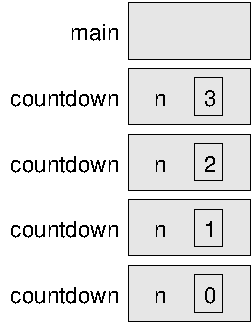
\includegraphics{stack2.pdf}

There is one frame for {\tt main} and four frames for {\tt countdown},
each with a different value for the parameter {\tt n}.  The bottom of
the stack, {\tt countdown} with {\tt n=0} is called the {\bf base
  case}.  It does not make a recursive call, so there are no more
frames for {\tt countdown}.

The frame for {\tt main} is empty because {\tt main} does not
have any parameters or variables.
